% Chapter 1
\chapter{Circuit Design and Analysis} % Write in your own chapter title
\label{Chapter3}
\lhead {Chapter 3. \emph{Circuit Design and Analysis}}
\section{Terminologies}
The average value of output load voltage is $V_{dc}$.
The average value of output load current is $I_{dc}$.
Thus, the output dc power:
$$P_{dc}=V_{dc}I_{dc}$$ 
The rms value of output load voltage is $V_{rms}$.
The rms value of output load current is $I_{rms}$.
Thus, the output ac power[3]:
\begin{equation}
P_{rms}=V_{rms}I_{rms}
\end{equation}
The efficiency of system is defined as
\begin{equation}
 \eta=\frac{P_{out}}{P_{in}}
\end{equation}
The effective rms(ac component) of output voltage can be calculated as:
\begin{equation}
V_{ac}=\sqrt[2]{V_{rms}^2-V_{dc}^2}
\end{equation}
The Form factor FF, describes the shape of output voltage as:
\begin{equation}
FF=\frac{V_{rms}}{V_{dc}}
\end{equation}
The Ripple factor RF,measures the ripple content of output voltage as:
\begin{equation}
RF=\frac{V_{ac}}{V_{dc}}
\end{equation}
Also,\\
\begin{equation}
RF=\sqrt[2]{FF^2-1}
\end{equation}
Next term is TUF (Transformer Utilization Factor) is defined as:
\begin{equation}
TUF=\frac{P_{dc}}{V_sI_s}
\end{equation}
where $V_s$ and $I_s$ are rms values of source voltage and current respectively.\\
The Displacement Factor DF is defined as;
\begin{equation}
DF=cos\phi
\end{equation}
where $\phi$ is the angle between fundamental component of input current and input voltage.This $\phi$ is known as Displacement angle.\\
The Harmonic factor HF of input current is defined as:
\begin{equation}
HF=\sqrt{(\frac{I_s}{I_{s1}})^2-1}
\end{equation}
where $I_{s1}$ is the fundamental component of input current $I_s$. Both are expressed in RMS.\\
The input Power factor PF is defined as:
\begin{equation}
PF=\frac{I_{s1}cos\phi}{I_s}
\end{equation}
Crest Factor CF which is of interest to specify the peak current ratings of devices and components is defined as:
 \begin{equation}
CF=\frac{I_{speak}}{I_s}
\end{equation}
where $I_{speak}$ is peak input current.\\
 Last one is THD Total Harmonic Distortion is measure harmonic distortion present in a signal and is defined as\\
 ``Ratio of sum of powers of all harmonic components to power of fundamental frequency.''
  \begin{equation}
THD=\frac{\sqrt{\sum_{i=2}^{n}V_i^2}}{V_1}
\end{equation}
\section{Design}
In general to obtain 9 levels in voltage waveform we need 4 cells of Independent H-Bridge.
But by using two independent sources of VDC1 = E and VDC2 = 3E we can obtain 9 levels in output voltage.In circuit \ref{fig:1} we have:
$$VDC1 = E$$\\
$$VDC2 = 3E$$
By applying specific sequence on switches s1, s2, s3, s4, s5, s6, s7 and s8 we can obtain voltage waveform with 9-levels
We only need to design sequences for s1, s3, s5 and s7, because we can apply inverted signal on other switches s4, s2, s8 and s6 respectively.
\begin{figure}[htbp]
	\centering
		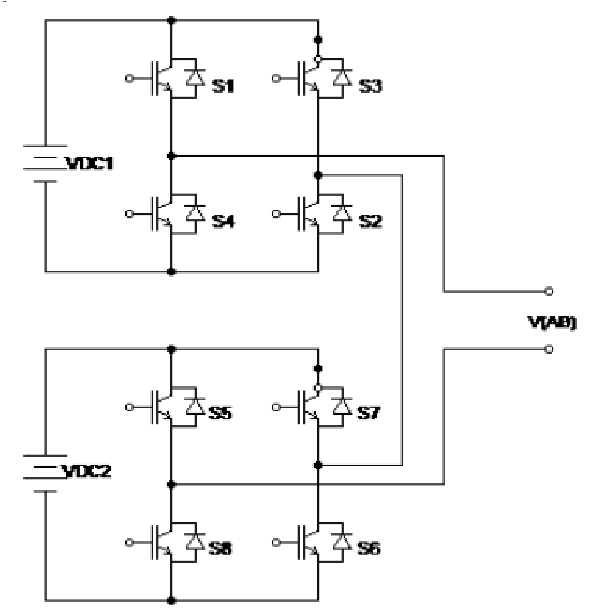
\includegraphics[width = 2.5in]{./Figures/design.pdf}
		\rule{35em}{5pt}
	\caption{H Bridge circuit for 9 Levels Voltage wave-forms}
	\label{fig:1}
\end{figure}

\begin{figure}[htbp]
	\centering
		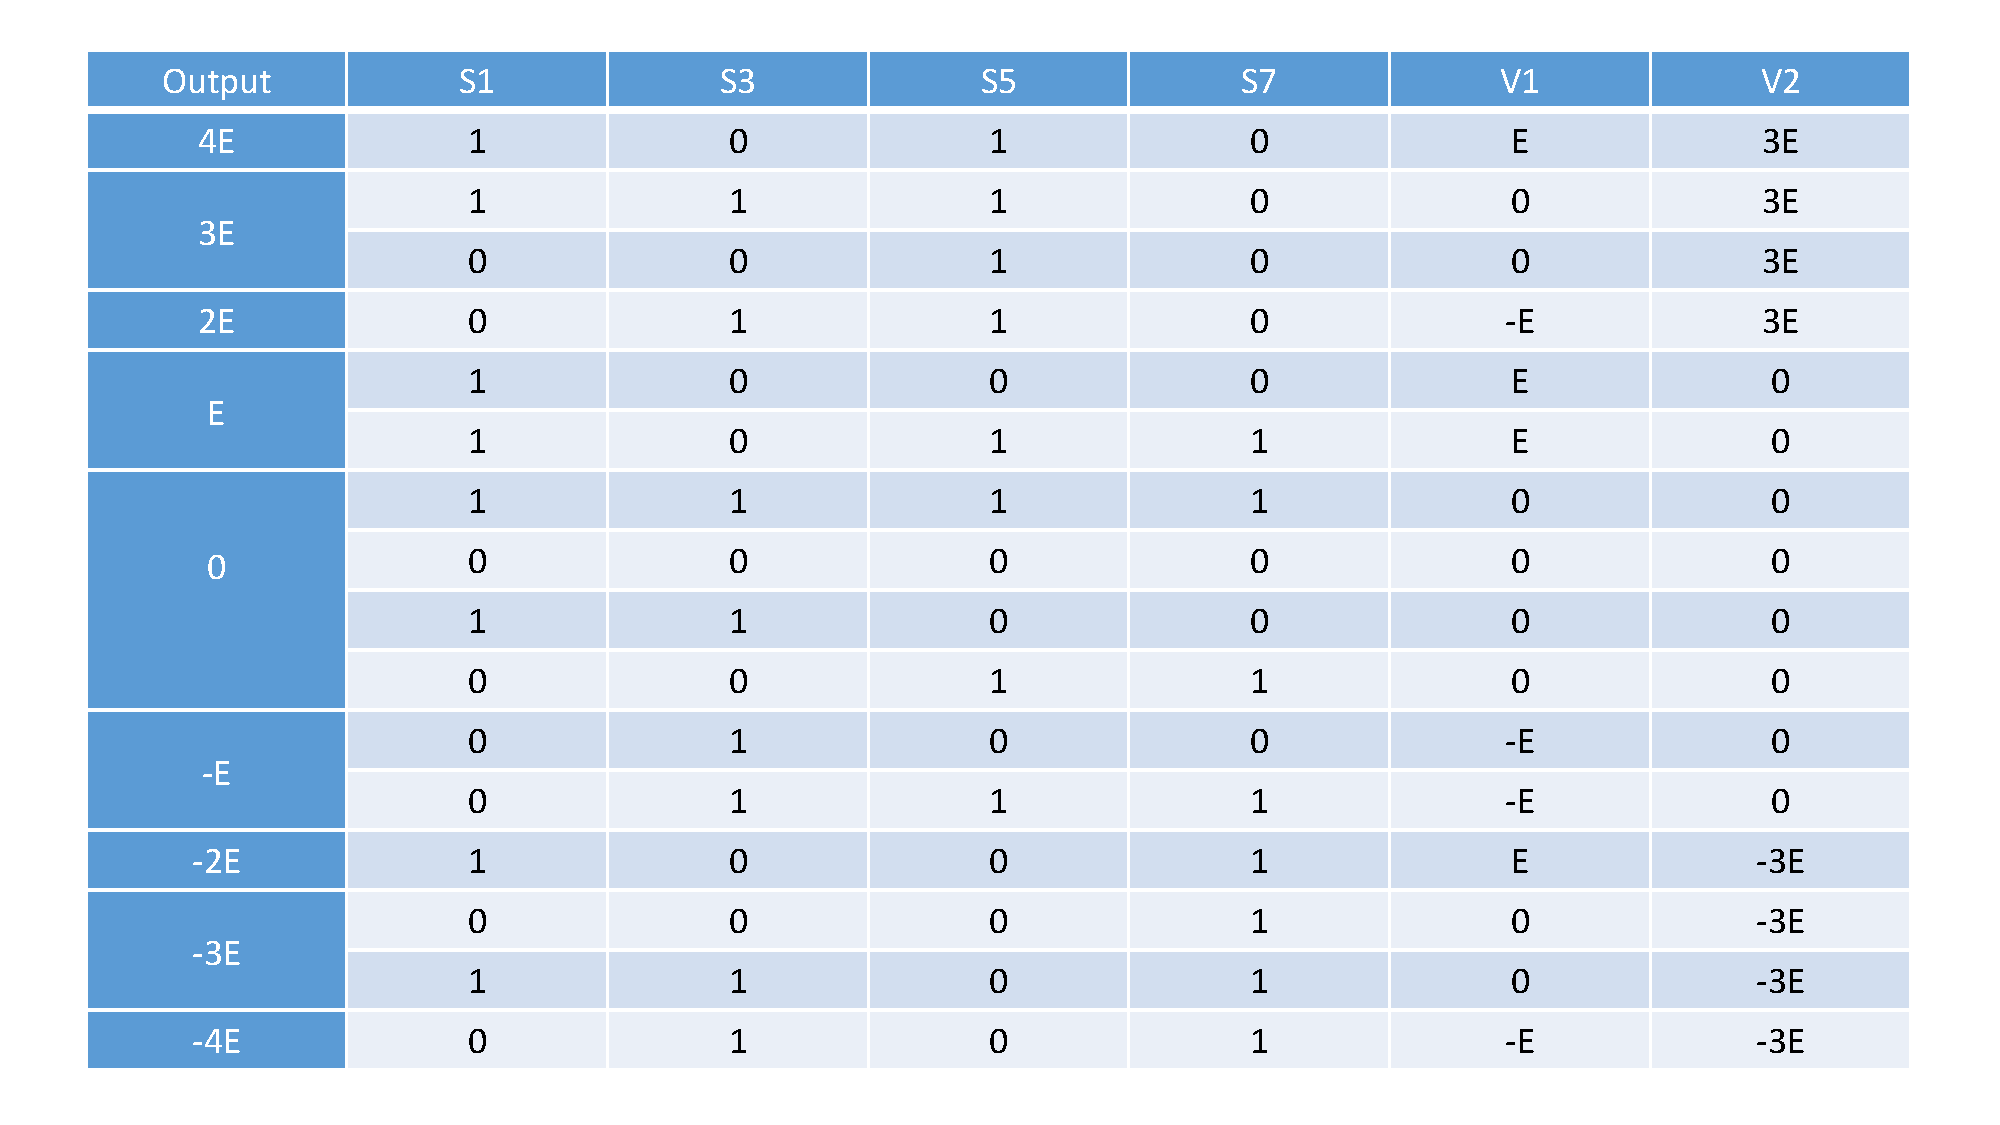
\includegraphics[width = 6in]{./Figures/SWITCH.pdf}
		\rule{35em}{5pt}
	\caption{Switching States for 9 Levels Voltage wave-forms}
	\label{fig:2}
\end{figure}
\begin{figure}[htbp]
	\centering
		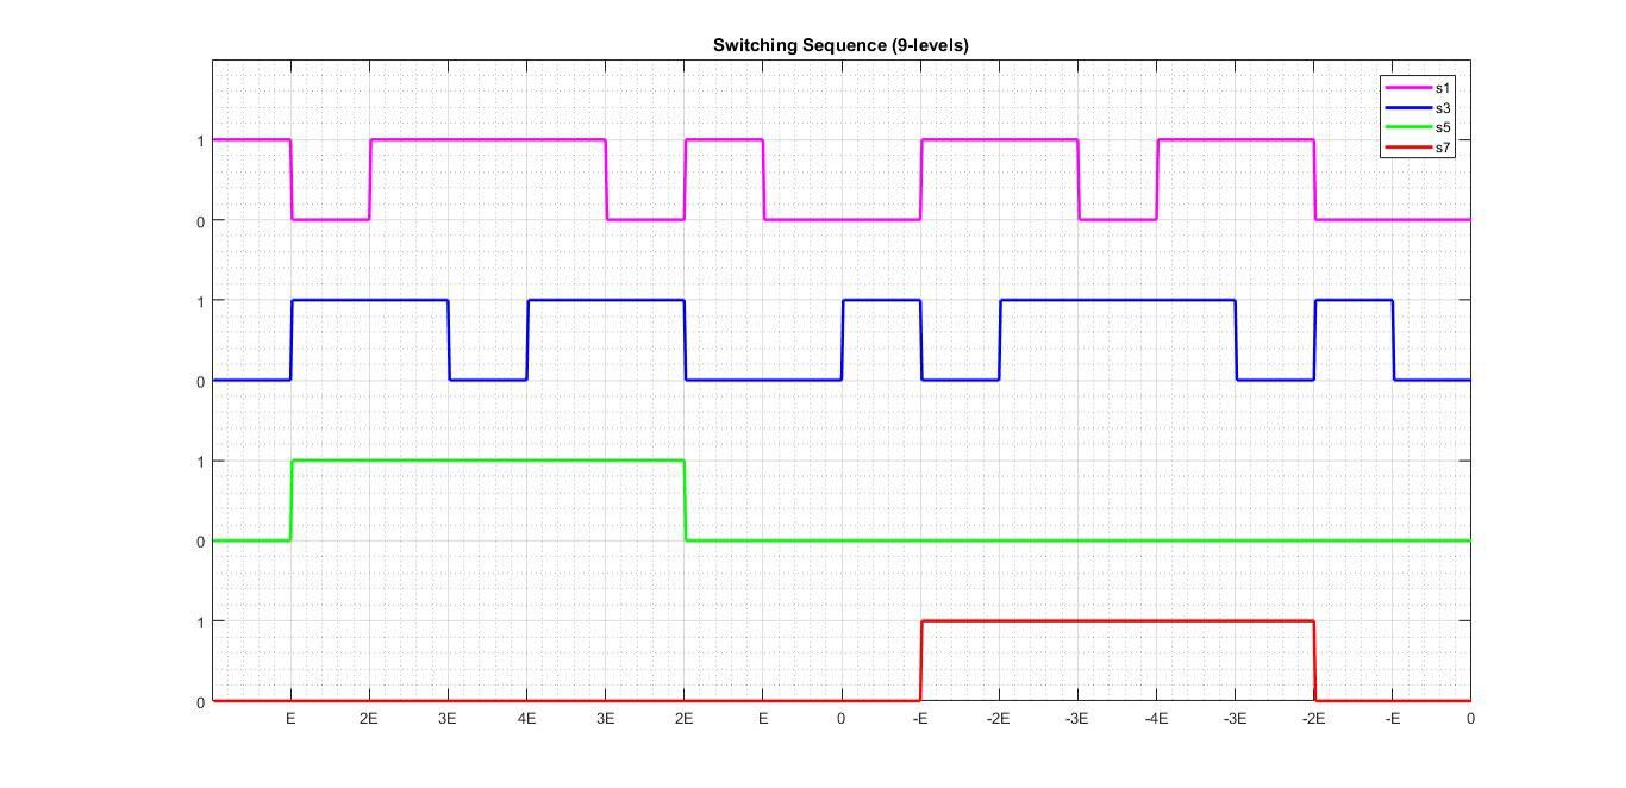
\includegraphics[width = 6in]{./Figures/graph.pdf}
		\rule{35em}{5pt}
	\caption{Graphical Representation of Switching Sequence with Minimum Transitions}
	\label{fig:3}
\end{figure}
By using switching states as shown in \ref{fig:3} we can define switching sequence.
The switching sequence is obtained by selecting switching states \ref{fig:2} so that minimum transitions occurs. 
By applying these sequences to respective switches s1, s3, s5 and s7 and inverted sequences on s4, s2, s8 and s6 respectively we get the output voltage waveform\ref{fig:4}.
To control output power we can use PWM techniques like Sinusoidal PWM as discussed before.
To control harmonics in output waveform we can change conduction angles.
\section{Analysis}
Lower frequency harmonics like 3, 5, 7, 9.. can be removed by choosing conduction angles wisely.
Higher frequency harmonics can be removed by filtering the output using Low Pass Filter.

The general Fourier series expression for ‘s’ steps in voltage waveform is given below:
\begin{figure}[htbp]
	\centering
		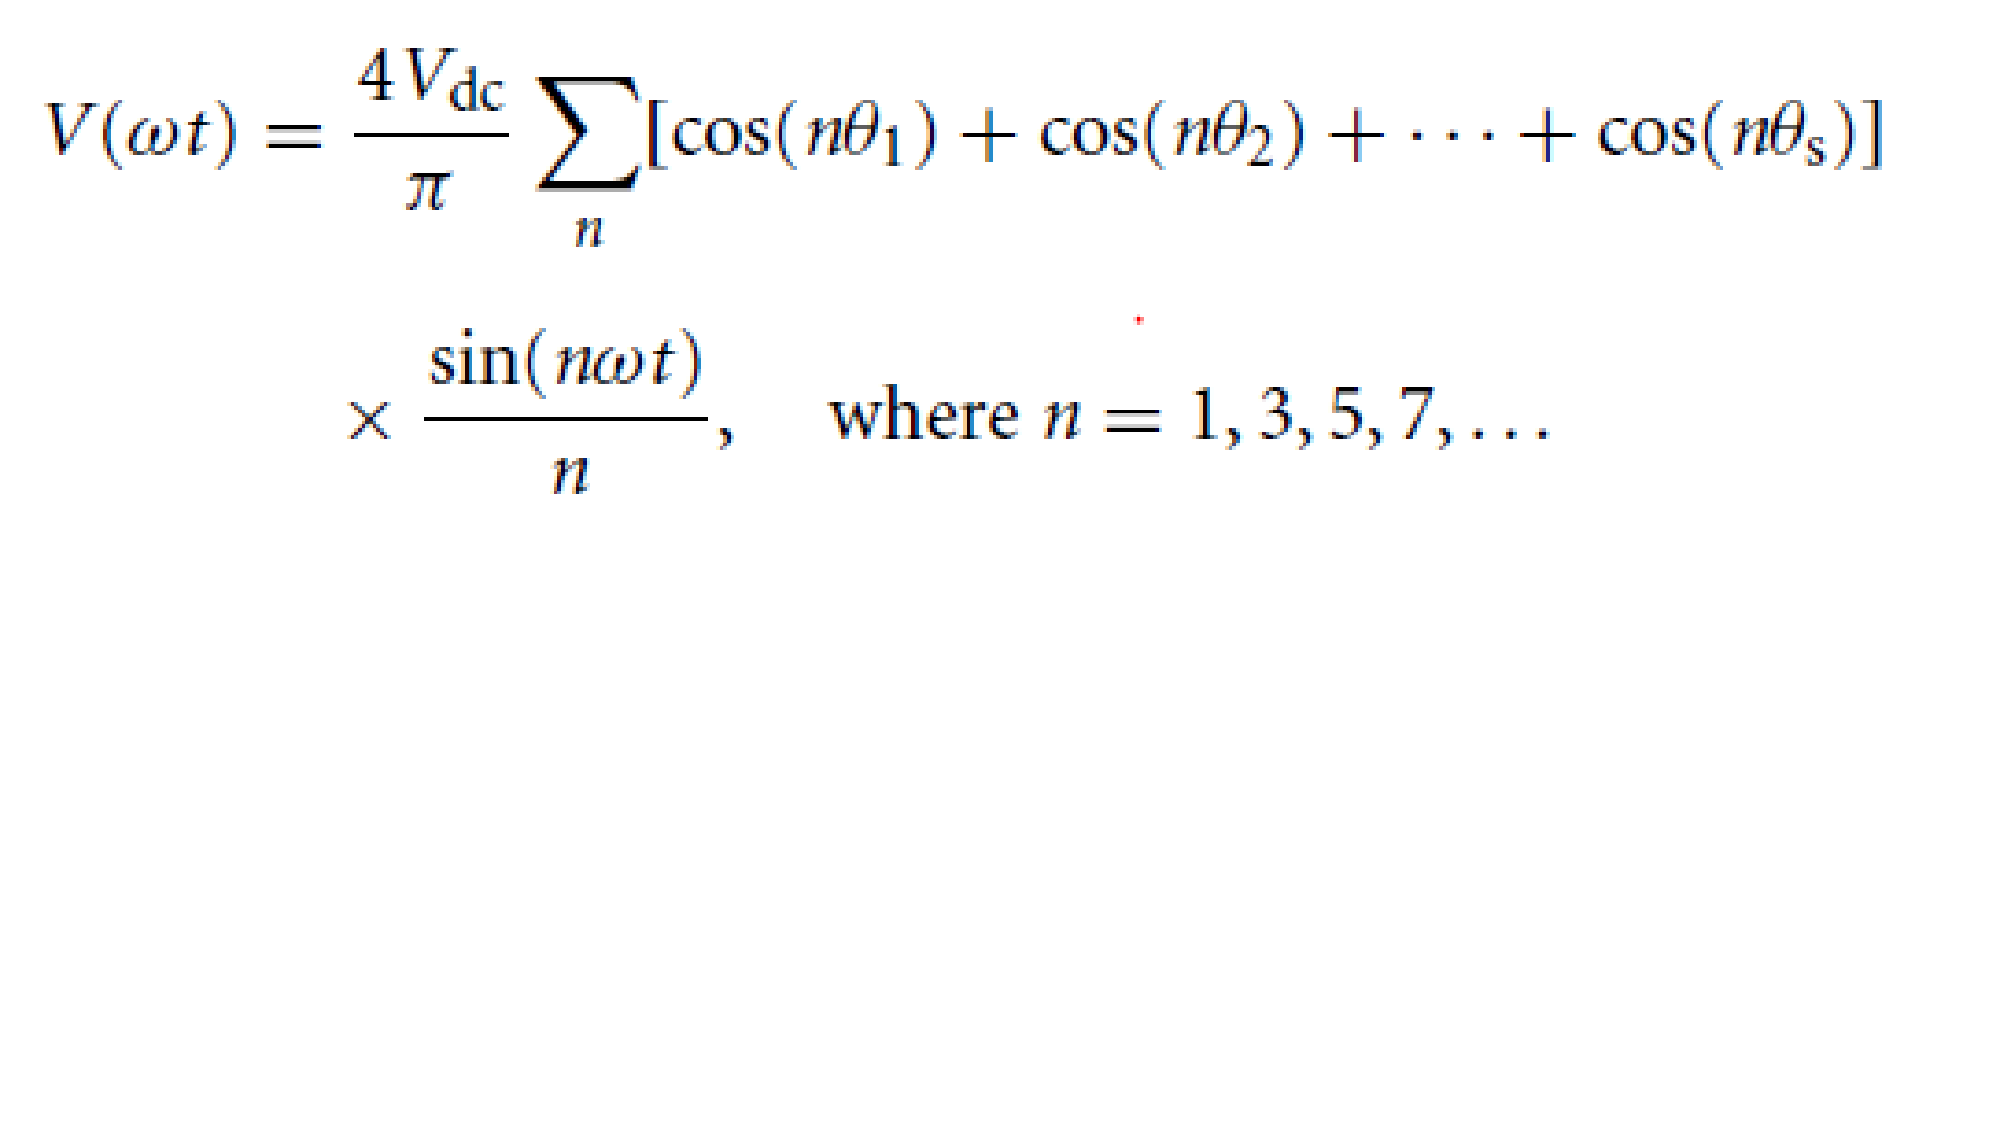
\includegraphics[width = 3.5in]{./Figures/eq.pdf}
				\end{figure}
				\begin{figure}[htbp]
\end{figure}
For $\theta1= 14.8^o, \theta2 = 30^o, \theta3 = 48^o and \theta4 = 68^o $ taken by hit and trial.The output\ref{fig:4} of 9 levels CHBMLI and its magnitude spectrum\ref{fig:5} is shown below. 
\begin{figure}[htbp]
	\centering
		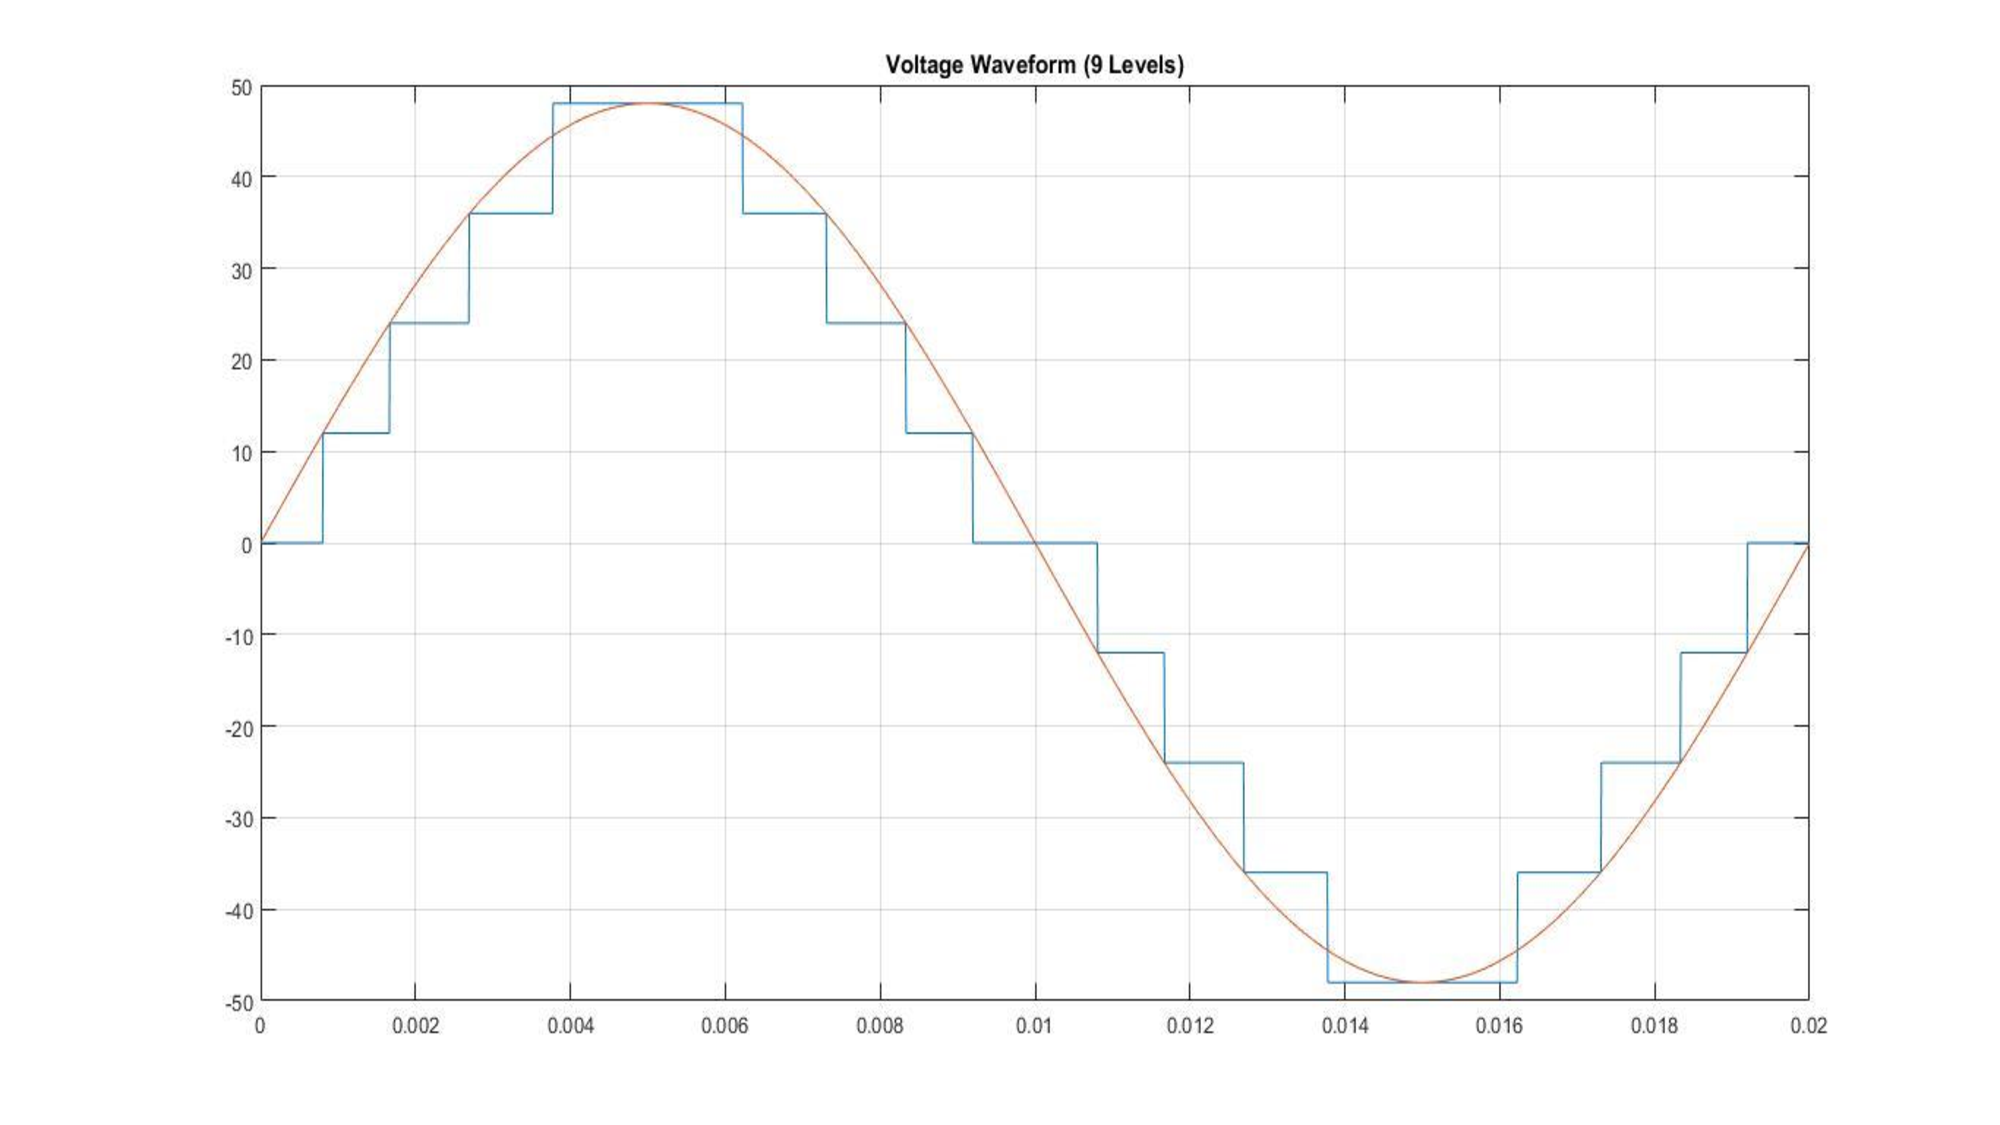
\includegraphics[width = 5in]{./Figures/Presentation5.pdf}
		\rule{35em}{5pt}
	\caption{9-Levels Voltage waveform when E=12 V}
	\label{fig:4}
\end{figure}
\begin{figure}[htbp]
	\centering
		\includegraphics[width = 5in]{./Figures/Spectrum.pdf}
		\rule{35em}{5pt}
	\caption{9-Levels Voltage Magnitude Spectrum}
	\label{fig:5}
\end{figure}
We can see form magnitude spectrum of output voltage that
\begin{itemize}
\item Fundamental component (f = 50Hz) has maximum contribution.
\item Even harmonics have zero contribution.
\item Odd harmonics are not zero, and 3rd harmonic (f = 150Hz) has maximum contribution after fundamental.
\end{itemize}
Contribution of fundamental component is:
$$V_1 = 31.023V$$also,$$ V_1 = 0.986Vo$$ 
where,
$$V_o=[\frac{4}{360}(\int_{14.8}^{30}E^2dt+\int_{30}^{48}4E^2dt+\int_{48}^{68}9E^2dt+\int_{68}^{90}E^2dt)]^{0.5}$$
$$V_o = 2.623E$$
$$V_o = 31.47V$$
Contribution of 3rd harmonic is:
$$V_3 = 3.6566V$$
$$V_3 = 0.116V_o$$
Contribution of 5th harmonic is:
$$V_5 = 0.1999V$$
$$V_5 = 0.006V_o$$
Contribution of 7th harmonic is:
$$V7 = 0.866V$$
$$V7 = 0.027V_o$$
Contribution of 9th harmonic is:
$$V_9 = 0.871V$$
$$V_9 = 0.027V_o$$
Thus,
$$THD=\frac{(V_{0}^{2}-V_{1}^{2})^{0.5}}{V_1}$$
$$THD=\frac{0.166V_o}{0.986V_o}$$
$$THD=16.9\%$$
We can change the conduction angles for better approximation of output waveform towards a sinusoidal waveform as shown fig\ref{fig:6} and fig\ref{fig:7} for $\theta1= 6^o, \theta2 = 22^o, \theta3 = 38^o and \theta4 = 60^o $ taken by hit and trial.
\begin{figure}[htbp]
	\centering
		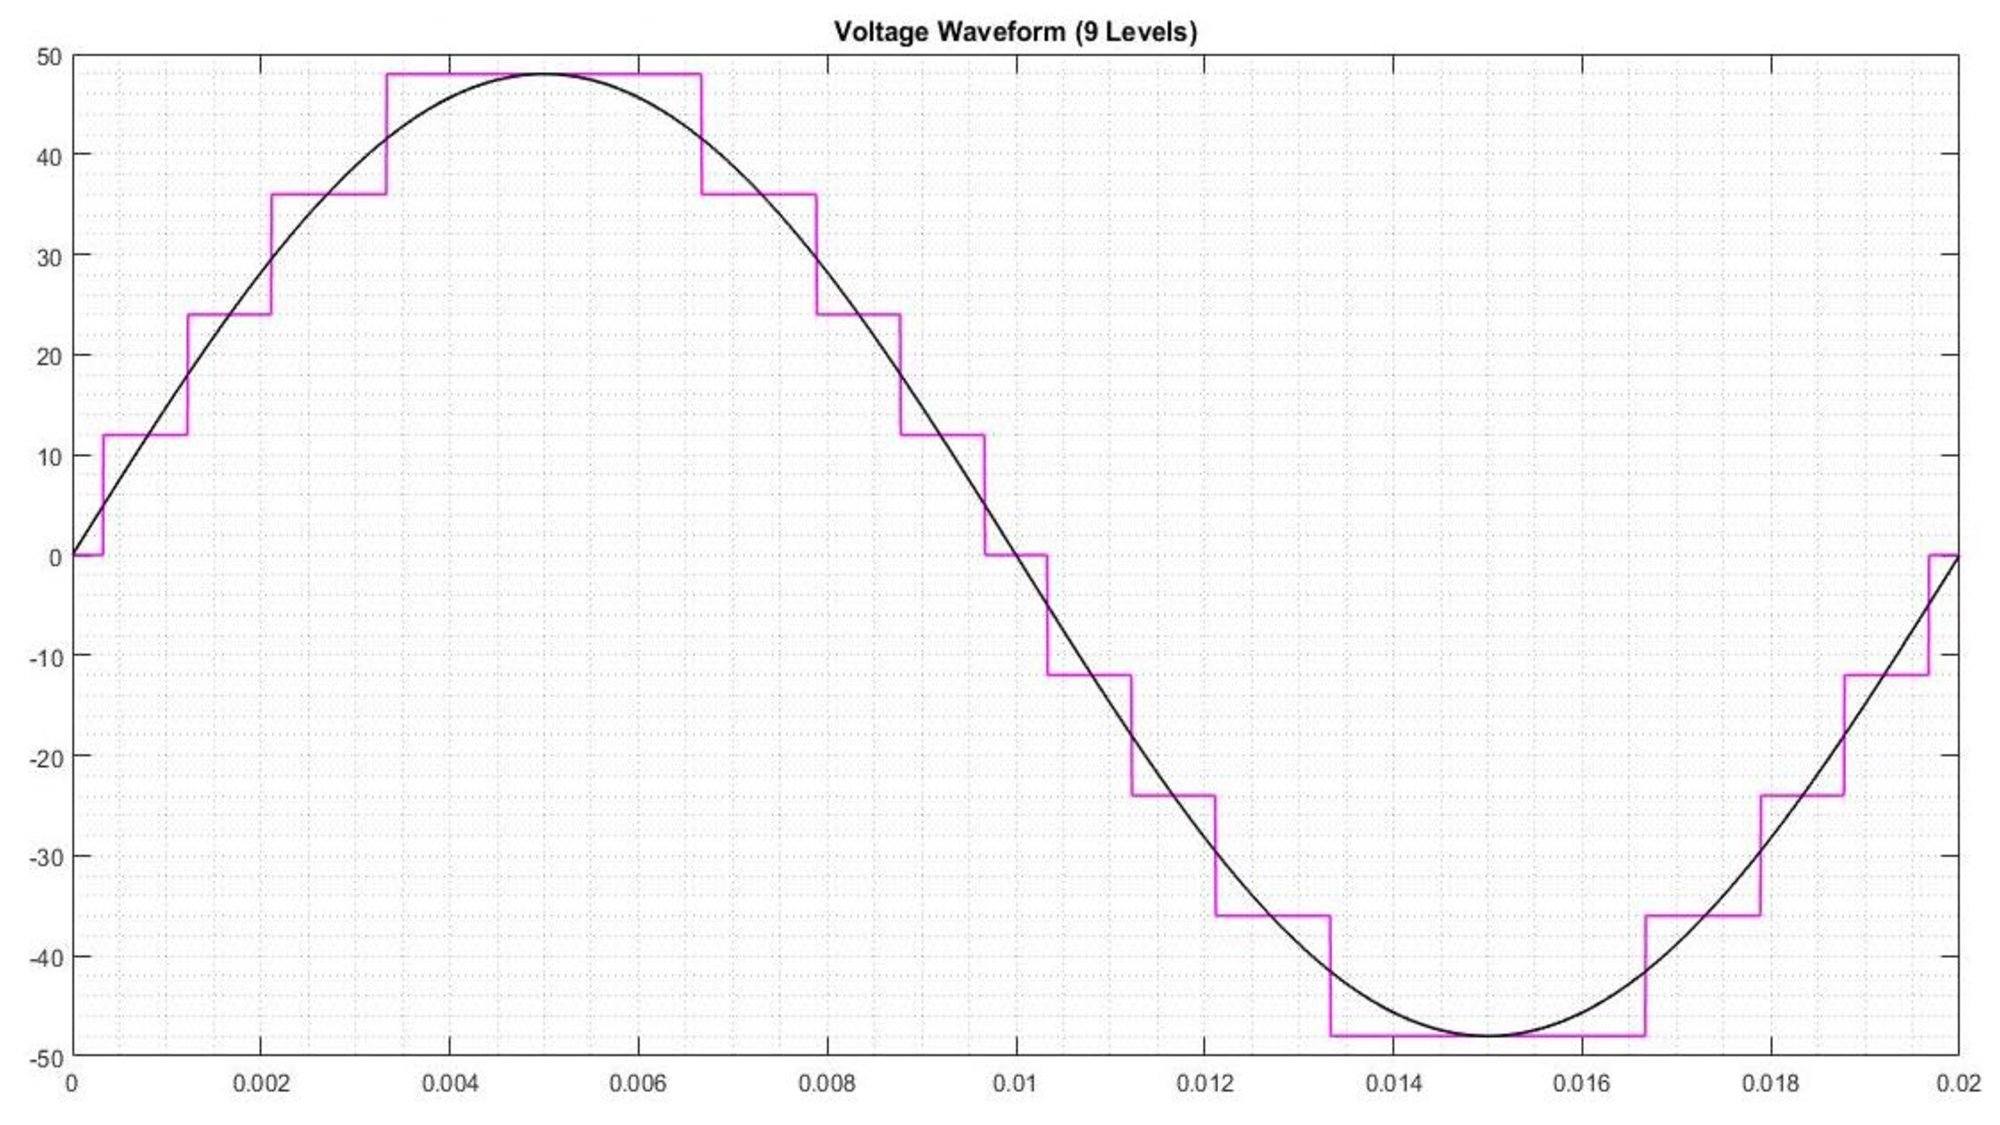
\includegraphics[width = 5in]{./Figures/better.pdf}
		\rule{35em}{5pt}
	\caption{Better Approximated 9 levels Voltage waveform}
	\label{fig:6}
\end{figure}
\begin{figure}[htbp]
	\centering
		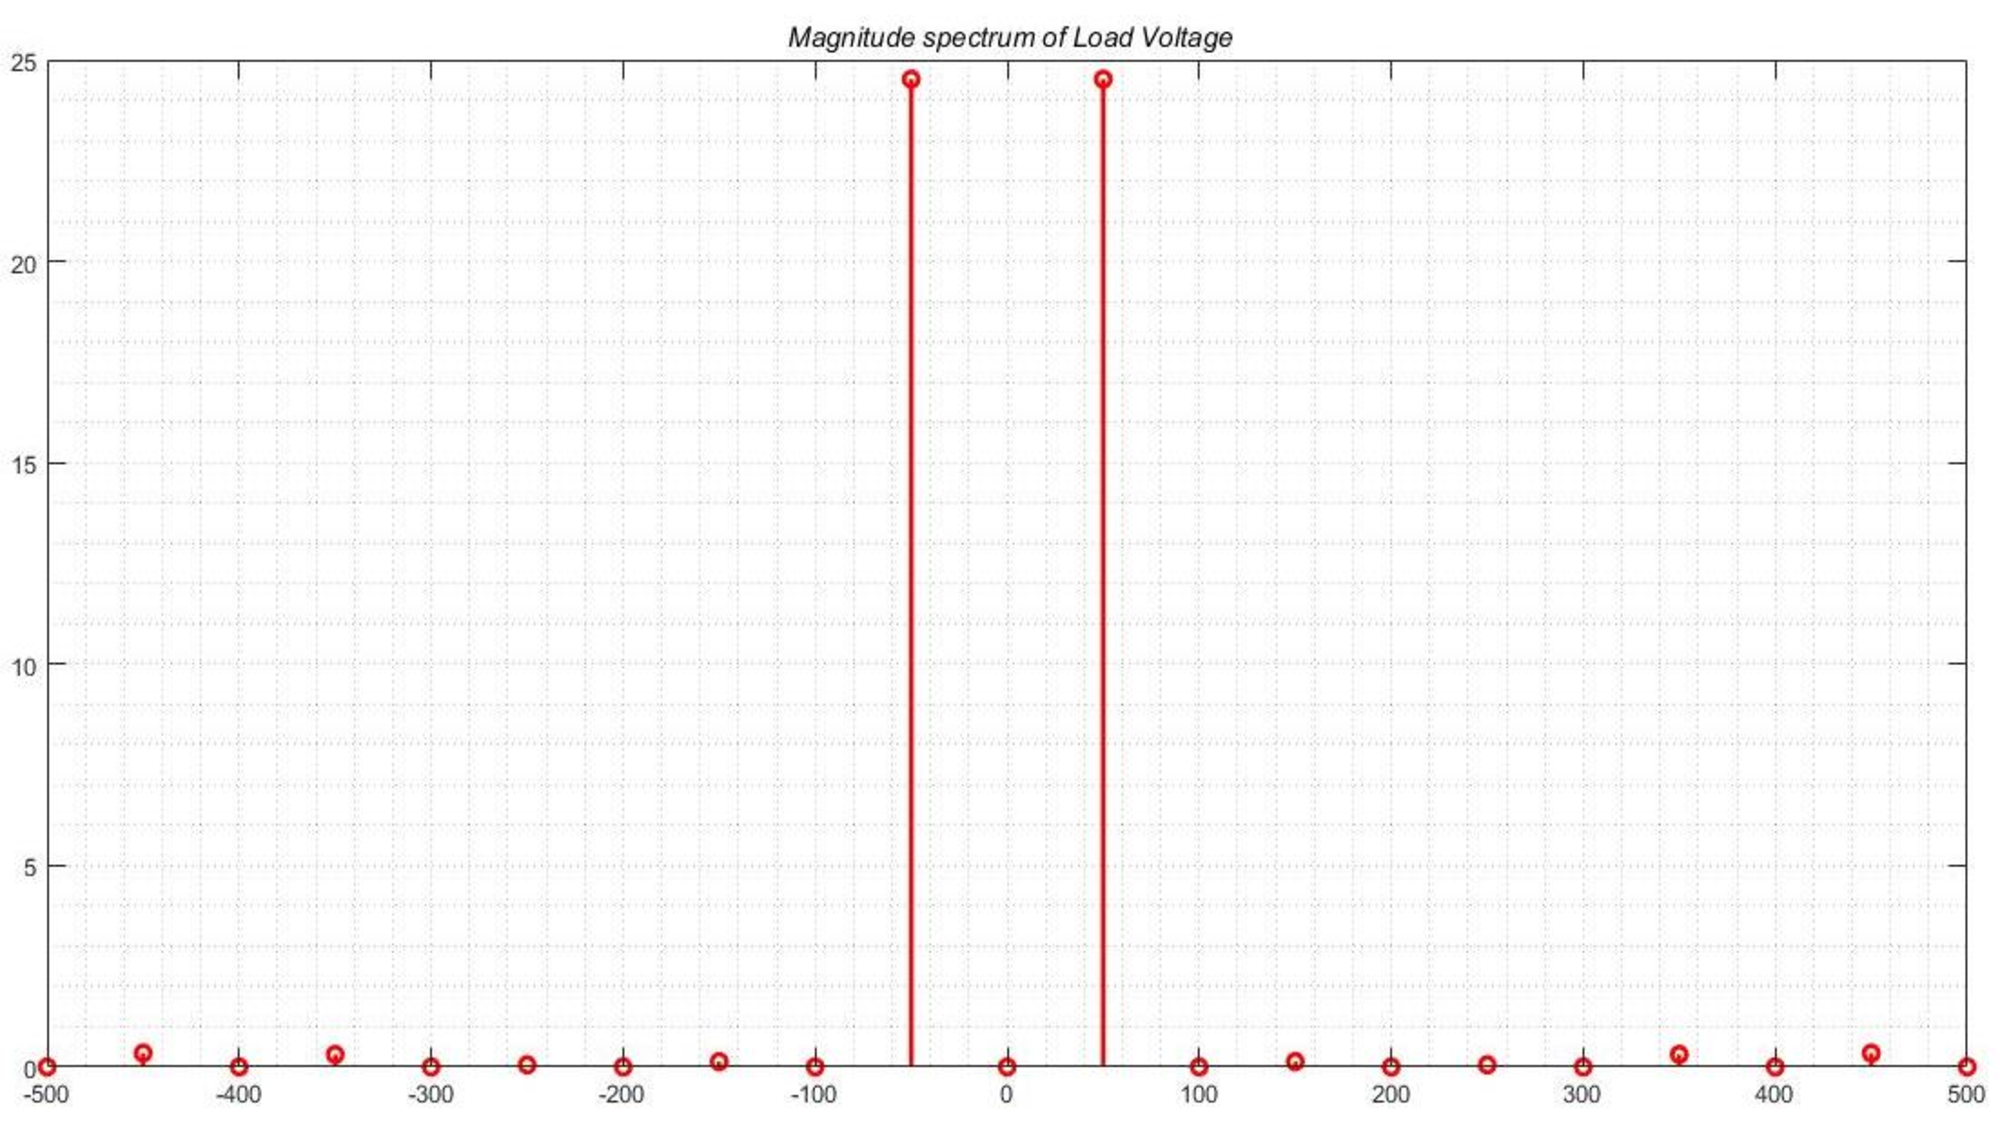
\includegraphics[width = 5in]{./Figures/imp.pdf}
		\rule{35em}{5pt}
	\caption{Improved Fourier Spectrum}
	\label{fig:7}
\end{figure}
$$V_o=[\frac{4}{360}(\int_{6}^{22}E^2dt+\int_{22}^{38}4E^2dt+\int_{38}^{60}9E^2dt+\int_{60}^{90}E^2dt)]^{0.5}$$
$$V_o = 2.901E$$
$$V_o = 34.82V$$
Contribution of fundamental component is:
$$V_1 = 34.68V$$
$$V_1 = 0.996V_o$$
Thus,
$$THD=\frac{(V_{0}^{2}-V_{1}^{2})^{0.5}}{V_1}$$
$$THD=\frac{0.0893V_o}{0.996V_o}$$
$$THD=8.97\%$$

\begin{center}
	\begin{tabular}{ |p{4cm}||p{4cm}|p{4cm}|  }
		\hline
		\multicolumn{3}{|c|}{Ratings} \\
		\hline
		Component & Voltage Rating & Current Rating\\
		\hline
		Isolated Supplies for Gate Driver & 15V & 0.3A\\
		TLP250 Input (Gate Driver) & 3.3V & 20mA\\
		TLP250 Output (Gate Driver) & 35V & 1.5A\\
		IRF450 (Switch) & 600V & 12A\\
		STM32F4 (GPIO Pins) & 3.3V & 20mA\\
		\hline
	\end{tabular}
\end{center}
